\chapter{Implementación}\label{cap:implementacion}

\section{Arquitectura general del sistema}\label{sec:arqui_sistema}
El sistema propuesto se organizó en dos módulos principales: un framework evolutivo y un simulador de SNN. Esta separación refleja explícitamente la distinción entre el algoritmo de búsqueda y la SNN con su dinámica. El framework evolutivo constituye la capa de algoritmos evolutivos, definición de problemas, manejo de población y registro de resultados, mientras que el simulador implementa la dinámica de la red, la codificación de datos en trenes de espigas y la decodificación para clasificación.

% El archivo platemo-cpp/CMakeLists.txt compila las fuentes de snn-simulator en una librería estática (snn\_libs) y las enlaza en el ejecutable principal platemo\_cpp, de modo que ambos módulos terminan formando un único binario con responsabilidades bien diferenciadas.

La arquitectura completa se puede describir como una secuencia de transformación desde la codificación del individuo hasta la evaluación de sus objetivos y el retorno al algoritmo evolutivo la cual se puede observar en la Figura \ref{fig:pipeline_snn_evo}.

\begin{itemize}
    \item Codificación: cada solución candidata se representa como un vector real de dimensión $D$, donde cada componente corresponde al peso de una sinapsis en el intervalo $[0,1]$.

    \item Construcción/decodificación de la SNN: el vector de pesos se proyecta sobre una topología fija.

    \item Simulación: el simulador codifica cada muestra de entrada en trenes de espigas, ejecuta la red paso a paso durante una ventana temporal fija y decodifica la salida mediante WTA.

    \item Evaluación: se calculan los dos objetivos: error y complejidad estructural.

    \item Retorno al algoritmo evolutivo: los objetivos se almacenan y el algoritmo multiobjetivo opera sobre ellos mediante ordenamiento no dominado y \textit{crowding distance}, sin necesidad de conocer los detalles internos de la simulación.
\end{itemize}

\begin{figure}[hbtp]
    \centering
    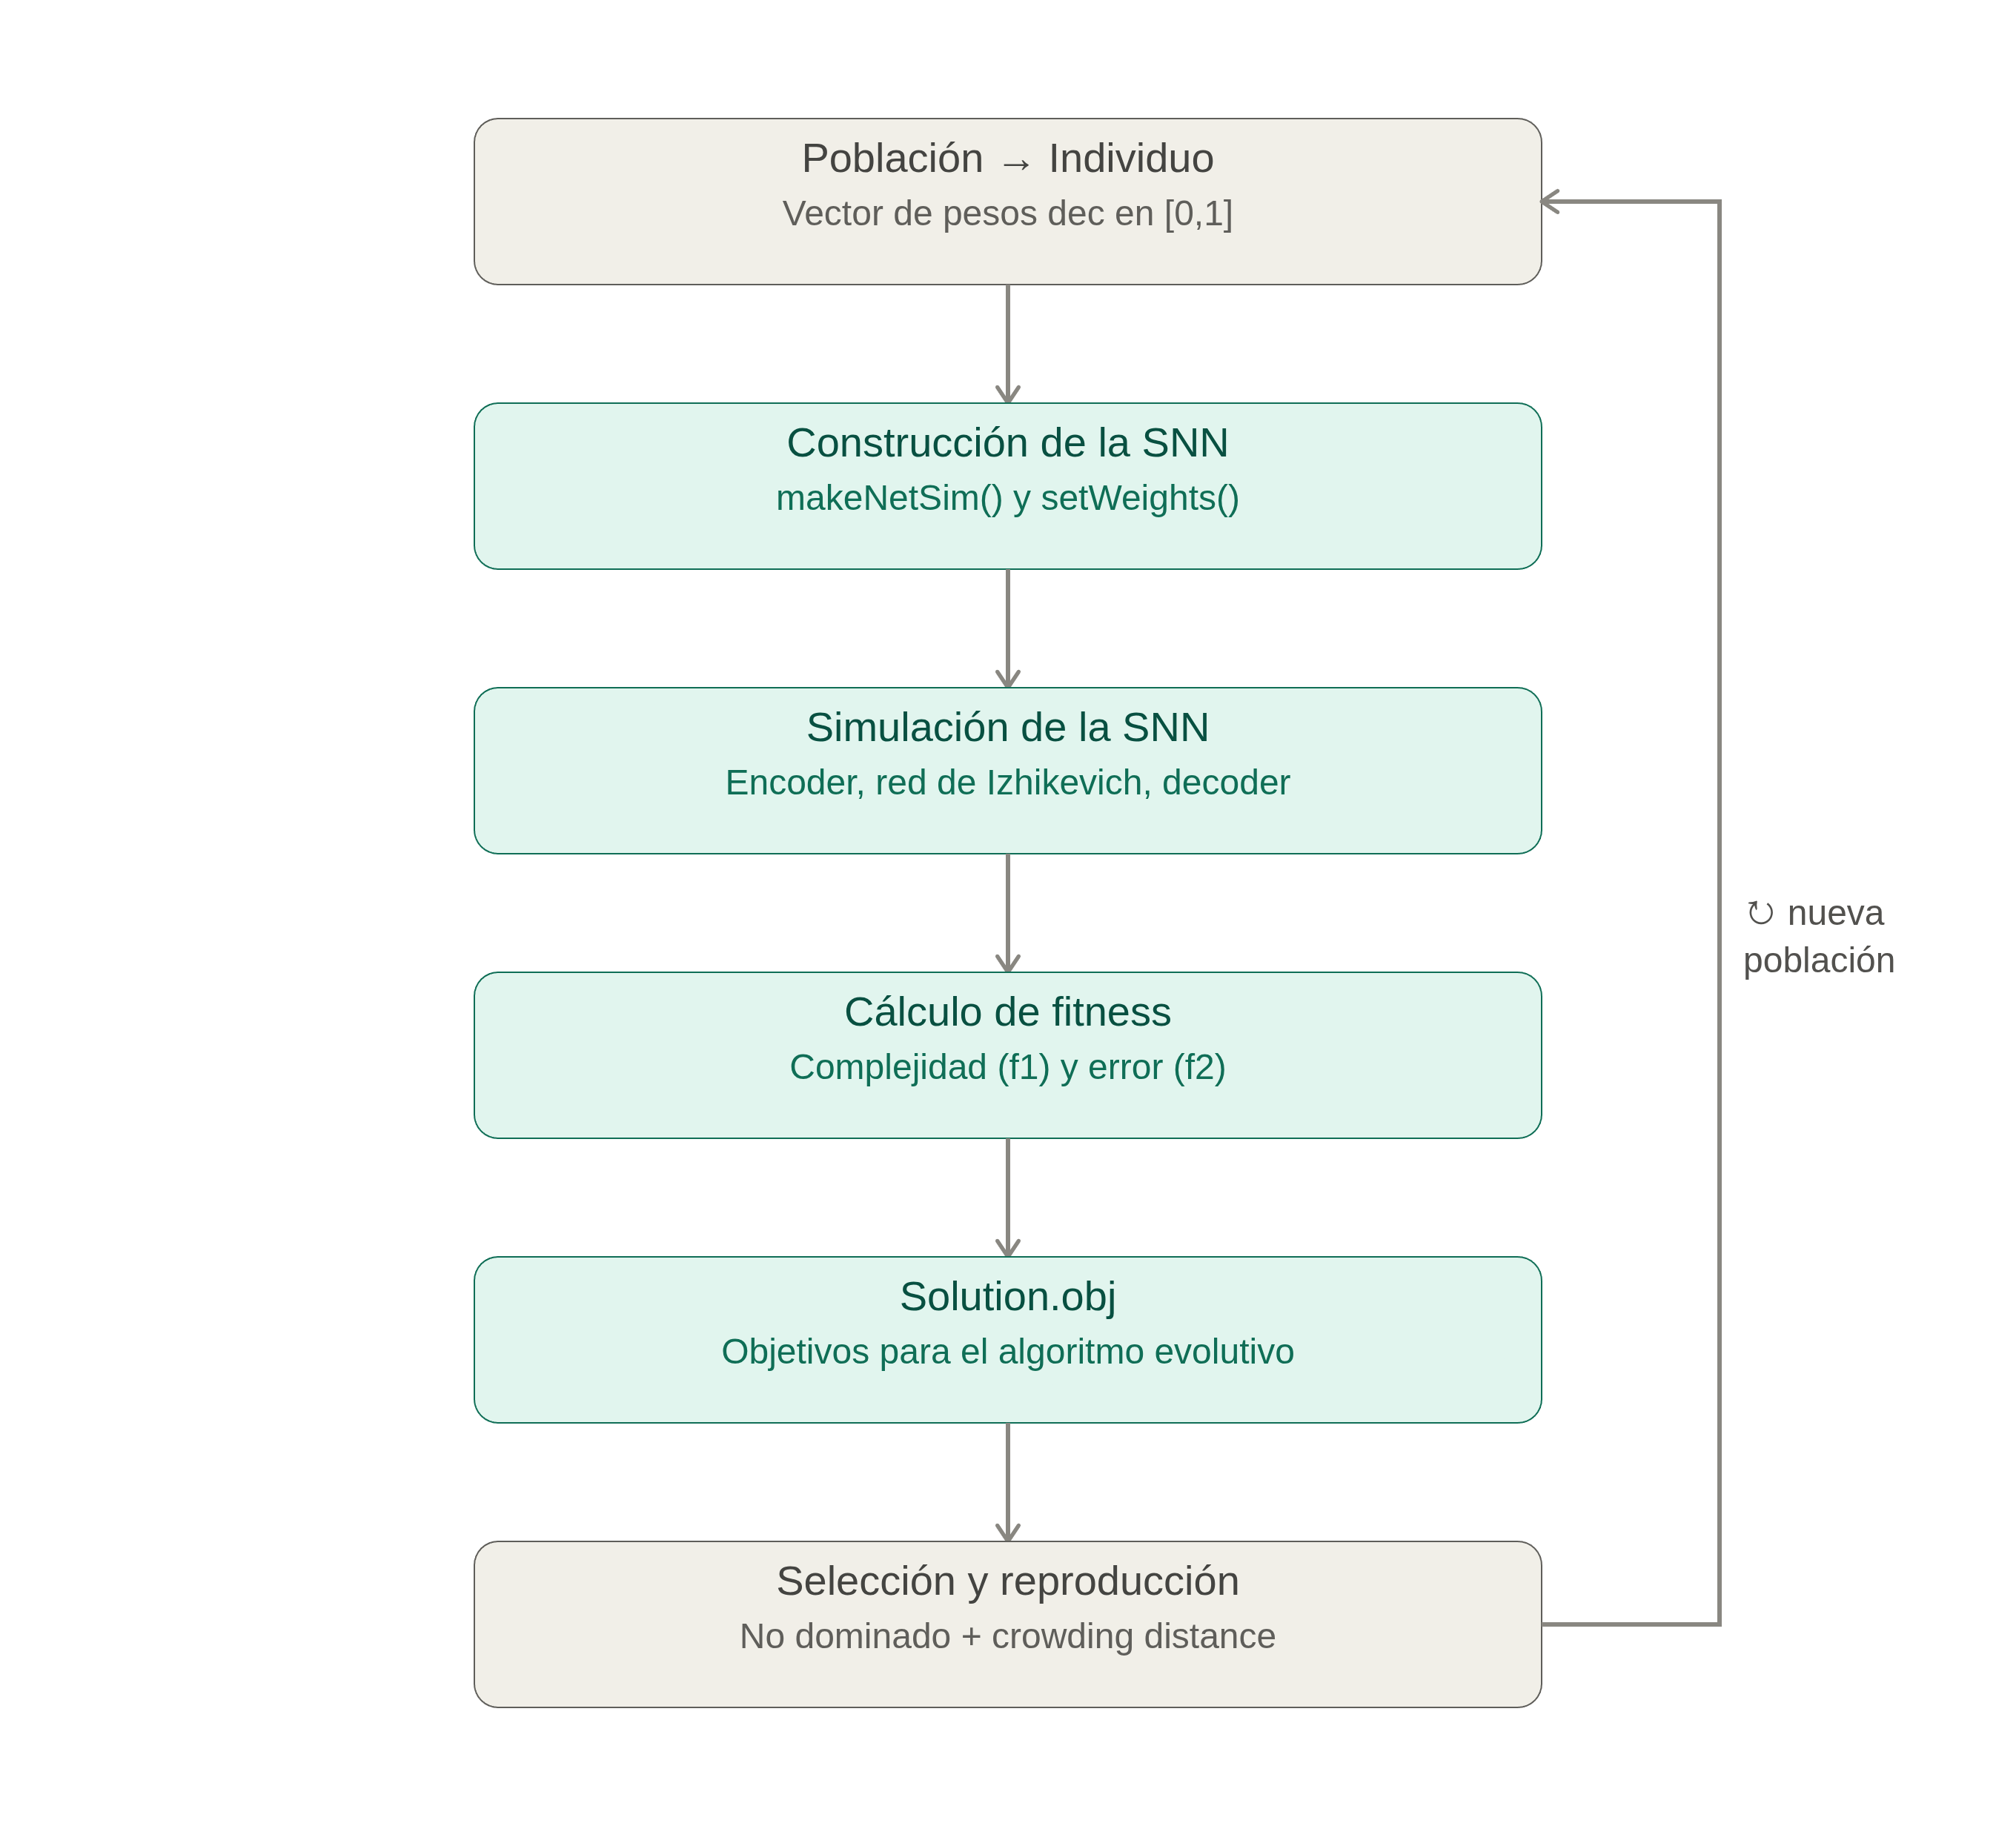
\includegraphics[width=0.75\linewidth]{images/pipeline_snn_evolutivo.png}
    \caption{Pipeline de evaluación del sistema evolutivo.}
    \label{fig:pipeline_snn_evo}
\end{figure}

\subsection{Flujo general de ejecución}
El ciclo evolutivo completo se instancia en el archivo principal del módulo evolutivo y sigue el patrón clásico población → inicialización → simulación/evaluación → selección → reproducción, repetido hasta agotar el presupuesto de evaluaciones. Este bucle define el flujo de información entre el módulo evolutivo y el simulador de SNN, garantizando tanto la coherencia de la evaluación multiobjetivo como la reproducibilidad de las corridas experimentales.

Durante la inicialización, se generan los pesos, produciendo aproximadamente un 50\% de ceros y sesgando la población inicial hacia redes esparsas. Sobre esta base común, cada algoritmo aplica una estrategia de arranque distinta: S-NSGA-II mediante VSSPS y MOEA-CKF mediante un Prior Analysis, ambas descritas en la Sección \ref{subsec:operadores_geneticos}.

En cada generación, todos los individuos se evalúan simulando la SNN sobre el conjunto de entrenamiento, en paralelo, aprovechando un pool de simuladores y redes preconstruidas por hilo. Una vez calculados los objetivos, ambos algoritmos utilizan selección por torneo binario para construir el mating pool\footnote{Conjunto de individuos seleccionados de la población actual para reproducirse.}, basada en el número de frente de Pareto y la distancia de aglomeración (\textit{crowding distance}), y posteriormente aplican selección ambiental tipo NSGA-II (ordenamiento no dominado + crowding) para decidir los individuos sobrevivientes tras fusionar padres e hijos. Esta etapa de selección es la única parte del ciclo generacional donde ambos algoritmos coinciden exactamente en su mecanismo.

La etapa de reproducción es, en cambio, donde S-NSGA-II y MOEA-CKF divergen con mayor fuerza, tal como se detalló en la Sección \ref{subsec:operadores_geneticos}. S-NSGA-II opera sobre un único vector real y aplica directamente sus operadores esparsos S-SBX y S-PM a todo el mating pool. MOEA-CKF, en cambio, divide la población en dos subgrupos en cada generación según la proporción $\rho$ y aplica a cada uno un procedimiento de reproducción distinto, guiado por reducción de dimensionalidad (PCA) y por agrupamiento de variables mediante \textit{k-means}, según se detalla en los pseudocódigos del Anexo \ref{chap:anexo-pseudo}.

El bucle generacional se ejecuta hasta que se alcanza el número máximo de evaluaciones \texttt{maxFE}; una vez terminada la evolución, se calcula el Hipervolumen (HV) del frente final y, opcionalmente, exporta el frente de Pareto, el historial de convergencia y los conteos de picos en el conjunto de test. El flujo general de ejecución, común en su estructura de alto nivel, pero con lógicas internas de inicialización y reproducción propias de cada algoritmo, se puede observar en la Figura \ref{fig:flujo_evo_511}.

\begin{figure}
    \centering
    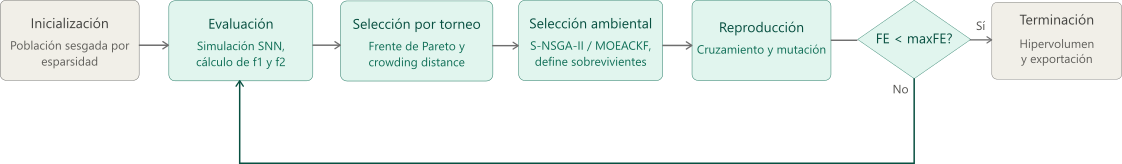
\includegraphics[width=1\linewidth]{images/flujo_evo_snn_horizontal.png}
    \caption{Flujo evolutivo generacional de alto nivel, común a ambos algoritmos en sus etapas de evaluación y selección. Las etapas de inicialización y reproducción encapsulan, bajo el mismo nombre, la lógica interna específica de S-NSGA-II y de MOEA-CKF. El ciclo repite evaluación mediante simulación de la SNN hasta que se cumple la condición de término $FE \geq maxFE$.}
    \label{fig:flujo_evo_511}
\end{figure}


\subsection{Módulos del sistema}
La implementación se organiza en torno a cinco módulos conceptuales que cubren la totalidad del pipeline: módulo evolutivo, simulador de SNN, manejo de datasets, métricas y configuración experimental. Esta separación en módulos permite mantener una arquitectura clara, donde el algoritmo evolutivo se mantiene independiente de los detalles del simulador y de la gestión de datos, facilitando la extensión y el análisis comparativo de algoritmos. Esta arquitectura modular se puede observar en la Figura \ref{fig:arquitectura_modular_sistema}.

El \textit{módulo evolutivo} define una jerarquía genérica Problema/Solución, implementa los dos algoritmos multiobjetivo y sus operadores genéticos. El \textit{simulador SNN} encapsula el modelo de neurona de Izhikevich, la estructura de la red (neuronas y sinapsis), el bucle de simulación temporal y los mecanismos de codificación y decodificación de spikes. A su vez, el \textit{módulo de datasets} se encarga de los archivos, la normalización, y la codificación de etiquetas. El \textit{módulo de métricas} las funciones objetivo y los indicadores agregados como el hipervolumen; finalmente, la \textit{configuración experimental} se gestiona íntegramente mediante scripts de orquestación.

\begin{figure}
    \centering
    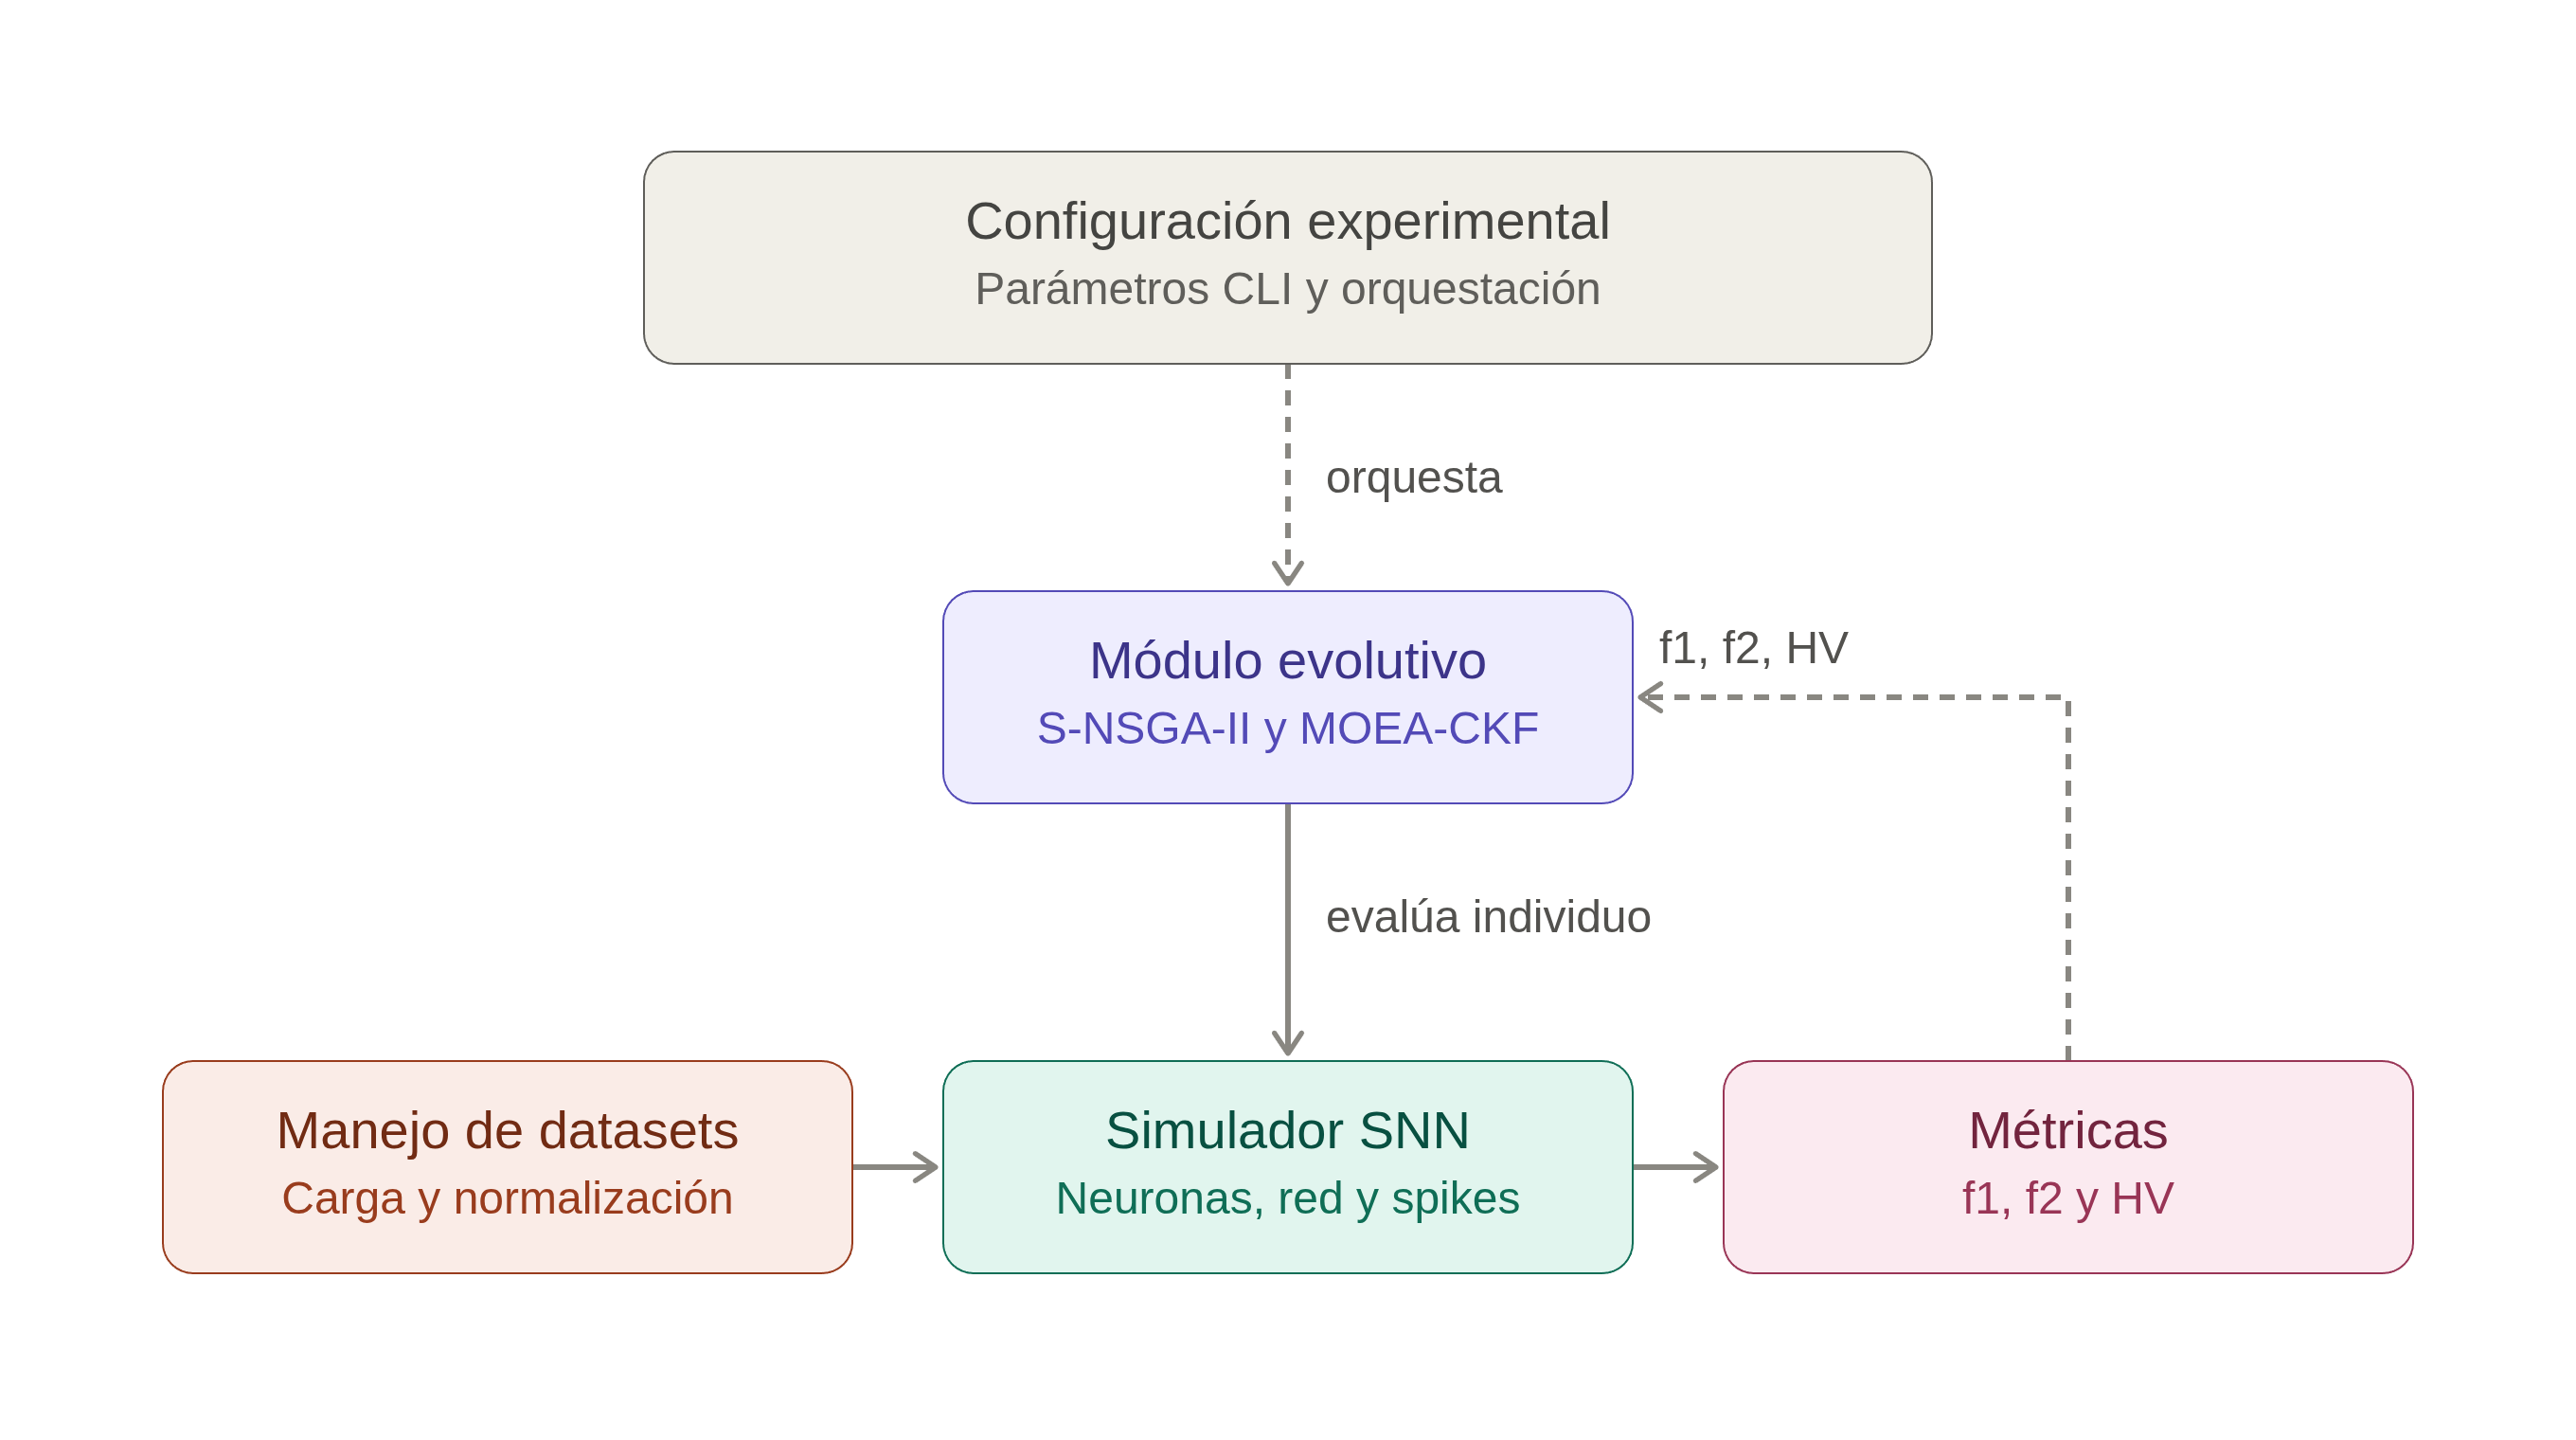
\includegraphics[width=0.7\linewidth]{images/modulos_sistema_snn.png}
    \caption{Arquitectura modular del sistema.}
    \label{fig:arquitectura_modular_sistema}
\end{figure}


%----------------------------

\section{Implementación de simulador SNN}\label{sec:simulador-snn}

El simulador SNN se implementó como un proyecto autónomo añadiendo además un framework de pruebas unitarias. La organización del código se estructura en módulos bien separados: núcleo de simulación (neurona, red, simulador), codificación de entrada, decodificación para clasificación y utilidades. Conceptualmente, la arquitectura sigue un pipeline Codificador → Red → Decodificador, donde un codificador transforma datos tabulares en trenes de espigas, la red de Izhikevich integra la dinámica neuronal y sináptica, y un decodificador de clasificación convierte los spikes de salida en decisiones y métricas de desempeño. El código fuente de este módulo está disponible como repositorio independiente en su repositorio: \url{https://github.com/Don-Uldaricio/snn-simulator}.

\subsection{Modelo neuronal y representación de la red}

Para esto, el simulador implementa exclusivamente neuronas de tipo Izhikevich, parametrizadas según el modelo original (ver \ref{sec:izhikevich}). La integración numérica se realiza mediante un esquema de Euler explícito con dos sub-pasos de tamaño $dt/2$ por paso de simulación, siguiendo la recomendación de Izhikevich para mejorar la estabilidad sin sacrificar eficiencia. La corriente total que recibe cada neurona combina conductancias excitatorias e inhibitorias con decaimiento exponencial, un término de corriente constante y un término de ruido uniforme generado con un RNG\footnote{Random Number Generator.}, lo que permite capturar variabilidad estocástica sin introducir condiciones de carrera.

Las conexiones sinápticas se representan mediante una estructura que almacena el índice de la neurona pre-sináptica, el índice de la neurona post-sináptica, una bandera que indica si la sinapsis es excitatoria o inhibitoria, y un peso escalar. A nivel de red, la topología se modela como una lista dispersa de sinapsis junto a listas de adyacencia pre-sinápticas y post-sinápticas (vectores de vectores de índices), lo que permite recorrer eficientemente las conexiones entrantes y salientes sin necesidad de matrices densas. El modelo no incorpora delays sinápticos explíctios ni conductancias por sinapsis: la transmisión de un spike es instantánea en el mismo paso de simulación y la dinámica de conductancias se implementa en las neuronas post-sinápticas.

\subsection{Motor de simulación y codificación}
El motor de simulación es la red, que mantiene vectores de neuronas Izhikevich y de sinapsis y ofrece métodos para avanzar la dinámica en el tiempo por pasos. En cada paso, el motor propaga las espigas generadas en el paso anterior actualizando las conductancias excitatorias e inhibitorias de las neuronas post-sinápticas, integra el estado de cada neurona y avanza el reloj global en un esquema de paso fijo, sin motor basado en eventos. El simulador envuelve a la red y a un codificador de entrada, gestionando la inyección de corrientes codificadas, la recolección de spikes y voltajes de salida, así como el cálculo de métricas como precisión, de modo que la simulación pueda utilizarse directamente como función objetivo en módulos externos de optimización. El módulo de codificación define dos implementaciones concretas: Poisson Encoder y TTFS (ver \ref{sec:codificacion-y-deco}).

\subsection{Validación y pruebas}
Se validó el simulador mediante una suite de 33 pruebas unitarias, implementadas con el framework Catch2 e integradas al sistema de compilación mediante CTest, lo que permite ejecutarlas de forma automatizada tras cada modificación del código fuente. Las pruebas se organizan según los mismos módulos conceptuales del simulador: núcleo, codificación y decodificación, tal como resume la Tabla \ref{tab:pruebas_simulador}.

\begin{table}[hbtp]
    \centering
    \small
    \caption{Distribución de las pruebas unitarias del simulador SNN por módulo.}
    \label{tab:pruebas_simulador}
    \begin{tabular}{lc}
        \toprule
        Módulo & N.º de pruebas \\
        \midrule
        Neurona (core/neuron) & 3 \\
        Red (core/network) & 7 \\
        Simulador (core/simulator) & 9 \\
        Codificación (encoding) & 9 \\
        Decodificación (decoding) & 5 \\
        \bottomrule
    \end{tabular}
\end{table}

En el núcleo, las pruebas sobre la neurona verificaron que una conductancia excitatoria sostenida produce disparos, que una conductancia inhibitoria de magnitud suficiente reduce el número de disparos respecto del caso puramente excitatorio, y que una corriente base constante ($i_{\text{offset}}$) es capaz de inducir disparos sin necesidad de estímulo externo. Sobre la red, las pruebas comprobaron la construcción correcta de la topología (conteo de neuronas, sinapsis, entradas y salidas), el almacenamiento y el peso de cada sinapsis, incluyendo asignación individual, masiva y homogénea, y la propagación efectiva de espigas a través de sinapsis excitatorias e inhibitorias en una red mínima de dos neuronas.

Sobre el simulador se probaron tanto la simulación con corriente directa (silencio total con corriente nula, disparos con corriente alta, y una entrada de tiempos de disparo por cada neurona de salida en el resultado) como la simulación con codificación de entrada, verificando que valores de entrada más altos producen más espigas en la salida. También se validaron las mutaciones de topología empleadas por los algoritmos evolutivos como inserción y eliminación de neuronas.

En codificación se probaron los dos esquemas implementados. El codificador de Poisson se validó verificando que un valor de entrada nulo no generaba espigas, que un valor alto generaba consistentemente al menos una espiga, que valores más altos producían más espigas que valores bajos bajo una ventana temporal, y que todos los tiempos de espiga generados caen dentro de la ventana de codificación. El codificador TTFS se validó comprobando que valores de entrada más altos generaban una espiga más temprana que valores bajos, y que un valor por debajo del umbral configurado no generaba espiga alguna.

En decodificación se probó unitariamente que el decodificador de clasificación seleccionaba la neurona de salida con mayor cantidad de espigas, que ante un empate en el conteo de espigas elegía una clase al azar entre las empatadas, y que normalizaba los puntajes por clase al intervalo $[0,1]$. Finalmente, se incluyen dos pruebas de integración extremo a extremo que combinan el Simulador y el Decodificador: una evalúa la exactitud de clasificación sobre un conjunto sintético de trece muestras con dos clases separables, exigiendo una exactitud mínima de 80\%, y otra evalúa la consistencia estadística de sobre diez repeticiones de una misma muestra codificada de forma estocástica, exigiendo que al menos ocho de diez repeticiones acierten la clase correcta.

Dado que los codificadores de Poisson y de tasa son estocásticos, varias pruebas emplean ventanas temporales prolongadas (hasta 500 ms) o repeticiones múltiples (10 corridas) para reducir la probabilidad de falsos negativos por variabilidad aleatoria, en lugar de fijar una semilla determinista para el generador de números aleatorios.

%  \subsection{Decisiones de diseño y evolución}
% Un aspecto central del diseño es que el simulador no implementa reglas de plasticidad internas como STDP, \textit{backpropagation through time} o gradientes sustitutos: la dinámica neuronal y sináptica es puramente forward, y el ajuste de pesos se delega expresamente al módulo externo de optimización evolutiva multiobjetivo, que utiliza el simulador como librería estática. Esta separación de responsabilidades permite mantener el simulador SNN pequeño, testeable y enfocado en la fidelidad de la dinámica de disparo, mientras que la exploración del espacio de pesos y topologías se aborda en un código independiente descrito en el capítulo dedicado a la optimización evolutiva.

%----------------------------------------------

\section{Implementación de algoritmos evolutivos}\label{sec:algoritmos-evolutivos}
Para la implementación de los algoritmos evolutivos aplicado al entrenamiento de SNN, se realizó la migración de los algoritmos desde la plataforma PlatEMO \cite{8065138_platEMO} a C++, cuya versión original se encuentra desarrollada en MATLAB. La migración se llevó a cabo procurando conservar la lógica original de las estructuras principales del código, incluyendo la representación de individuos, la inicialización de la población, los operadores genéticos, los mecanismos de selección y el procedimiento de actualización generacional. En aquellos casos en que ciertas funciones o utilidades de MATLAB no contaban con un equivalente directo en C++, se desarrollaron implementaciones alternativas que mantuvieran un comportamiento funcionalmente equivalente dentro del algoritmo. Estos casos correspondieron principalmente a funciones nativas o de \textit{toolbox} de MATLAB sin contraparte en la biblioteca estándar de C++ ni en Eigen (\texttt{unique(...,'rows')}, \texttt{sortrows}, \texttt{pdist2} o \texttt{kmeans}) y a las funciones de generación de números aleatorios (\texttt{randi}, \texttt{randperm}, \texttt{unifrnd}), cuyo generador difiere entre ambas plataformas. La Tabla \ref{tab:funciones_sin_equivalente} detalla estos casos y la estrategia de reimplementación adoptada en cada uno. En la Tabla \ref{tab:fidelidad_algoritmos} se muestra un resumen de la fidelidad de la migración de los SMOEA a C++. El código fuente de este módulo está disponible como repositorio independiente (ver Anexo \ref{chap:anexo-repos}).

% En este caso, S-NSGA-II corresponde al algoritmo con mayor fidelidad respecto de la implementación original, debido a que sus operadores presentan una lógica más directa de traducir que los componentes de MOEA-CKF.

Dado que MATLAB y C++ implementan generadores de números pseudoaleatorios distintos, no fue posible reproducir de forma idéntica, número a número, la traza de ejecución de un algoritmo estocástico entre ambas implementaciones. Por esta razón, la equivalencia entre las versiones MATLAB y C++ de cada operador no se validó comparando las salidas numéricas de ejecuciones específicas, sino a nivel de la construcción matemática y algorítmica de cada componente: se verificó que cada función migrada implementara la misma definición matemática, el mismo criterio de orden lexicográfico, o el mismo procedimiento discreto que su contraparte original (por ejemplo, el muestreo uniforme con o sin reemplazo de \texttt{randperm}/\texttt{randi}). Esta fue, por tanto, una validación de equivalencia funcional por construcción y no una validación empírica de igualdad de resultados entre plataformas, lo cual se reconoce como una limitación metodológica del proceso de migración.

Con el fin de facilitar la mantenibilidad y la validación del sistema, la implementación se organizó de forma modular al igual que en el código original. Se separaron los componentes asociados a la codificación de soluciones, los operadores genéticos, la evaluación del desempeño de la población y la interfaz de comunicación con el simulador de SNN. Esta organización permitió desacoplar la lógica propia de cada algoritmo evolutivo de la lógica de simulación neuronal, favoreciendo la reutilización de componentes en distintas configuraciones experimentales. La Figura \ref{fig:modulos_platemo_cpp} muestra esta organización interna del módulo evolutivo.

\begin{figure}[hbtp]
    \centering
    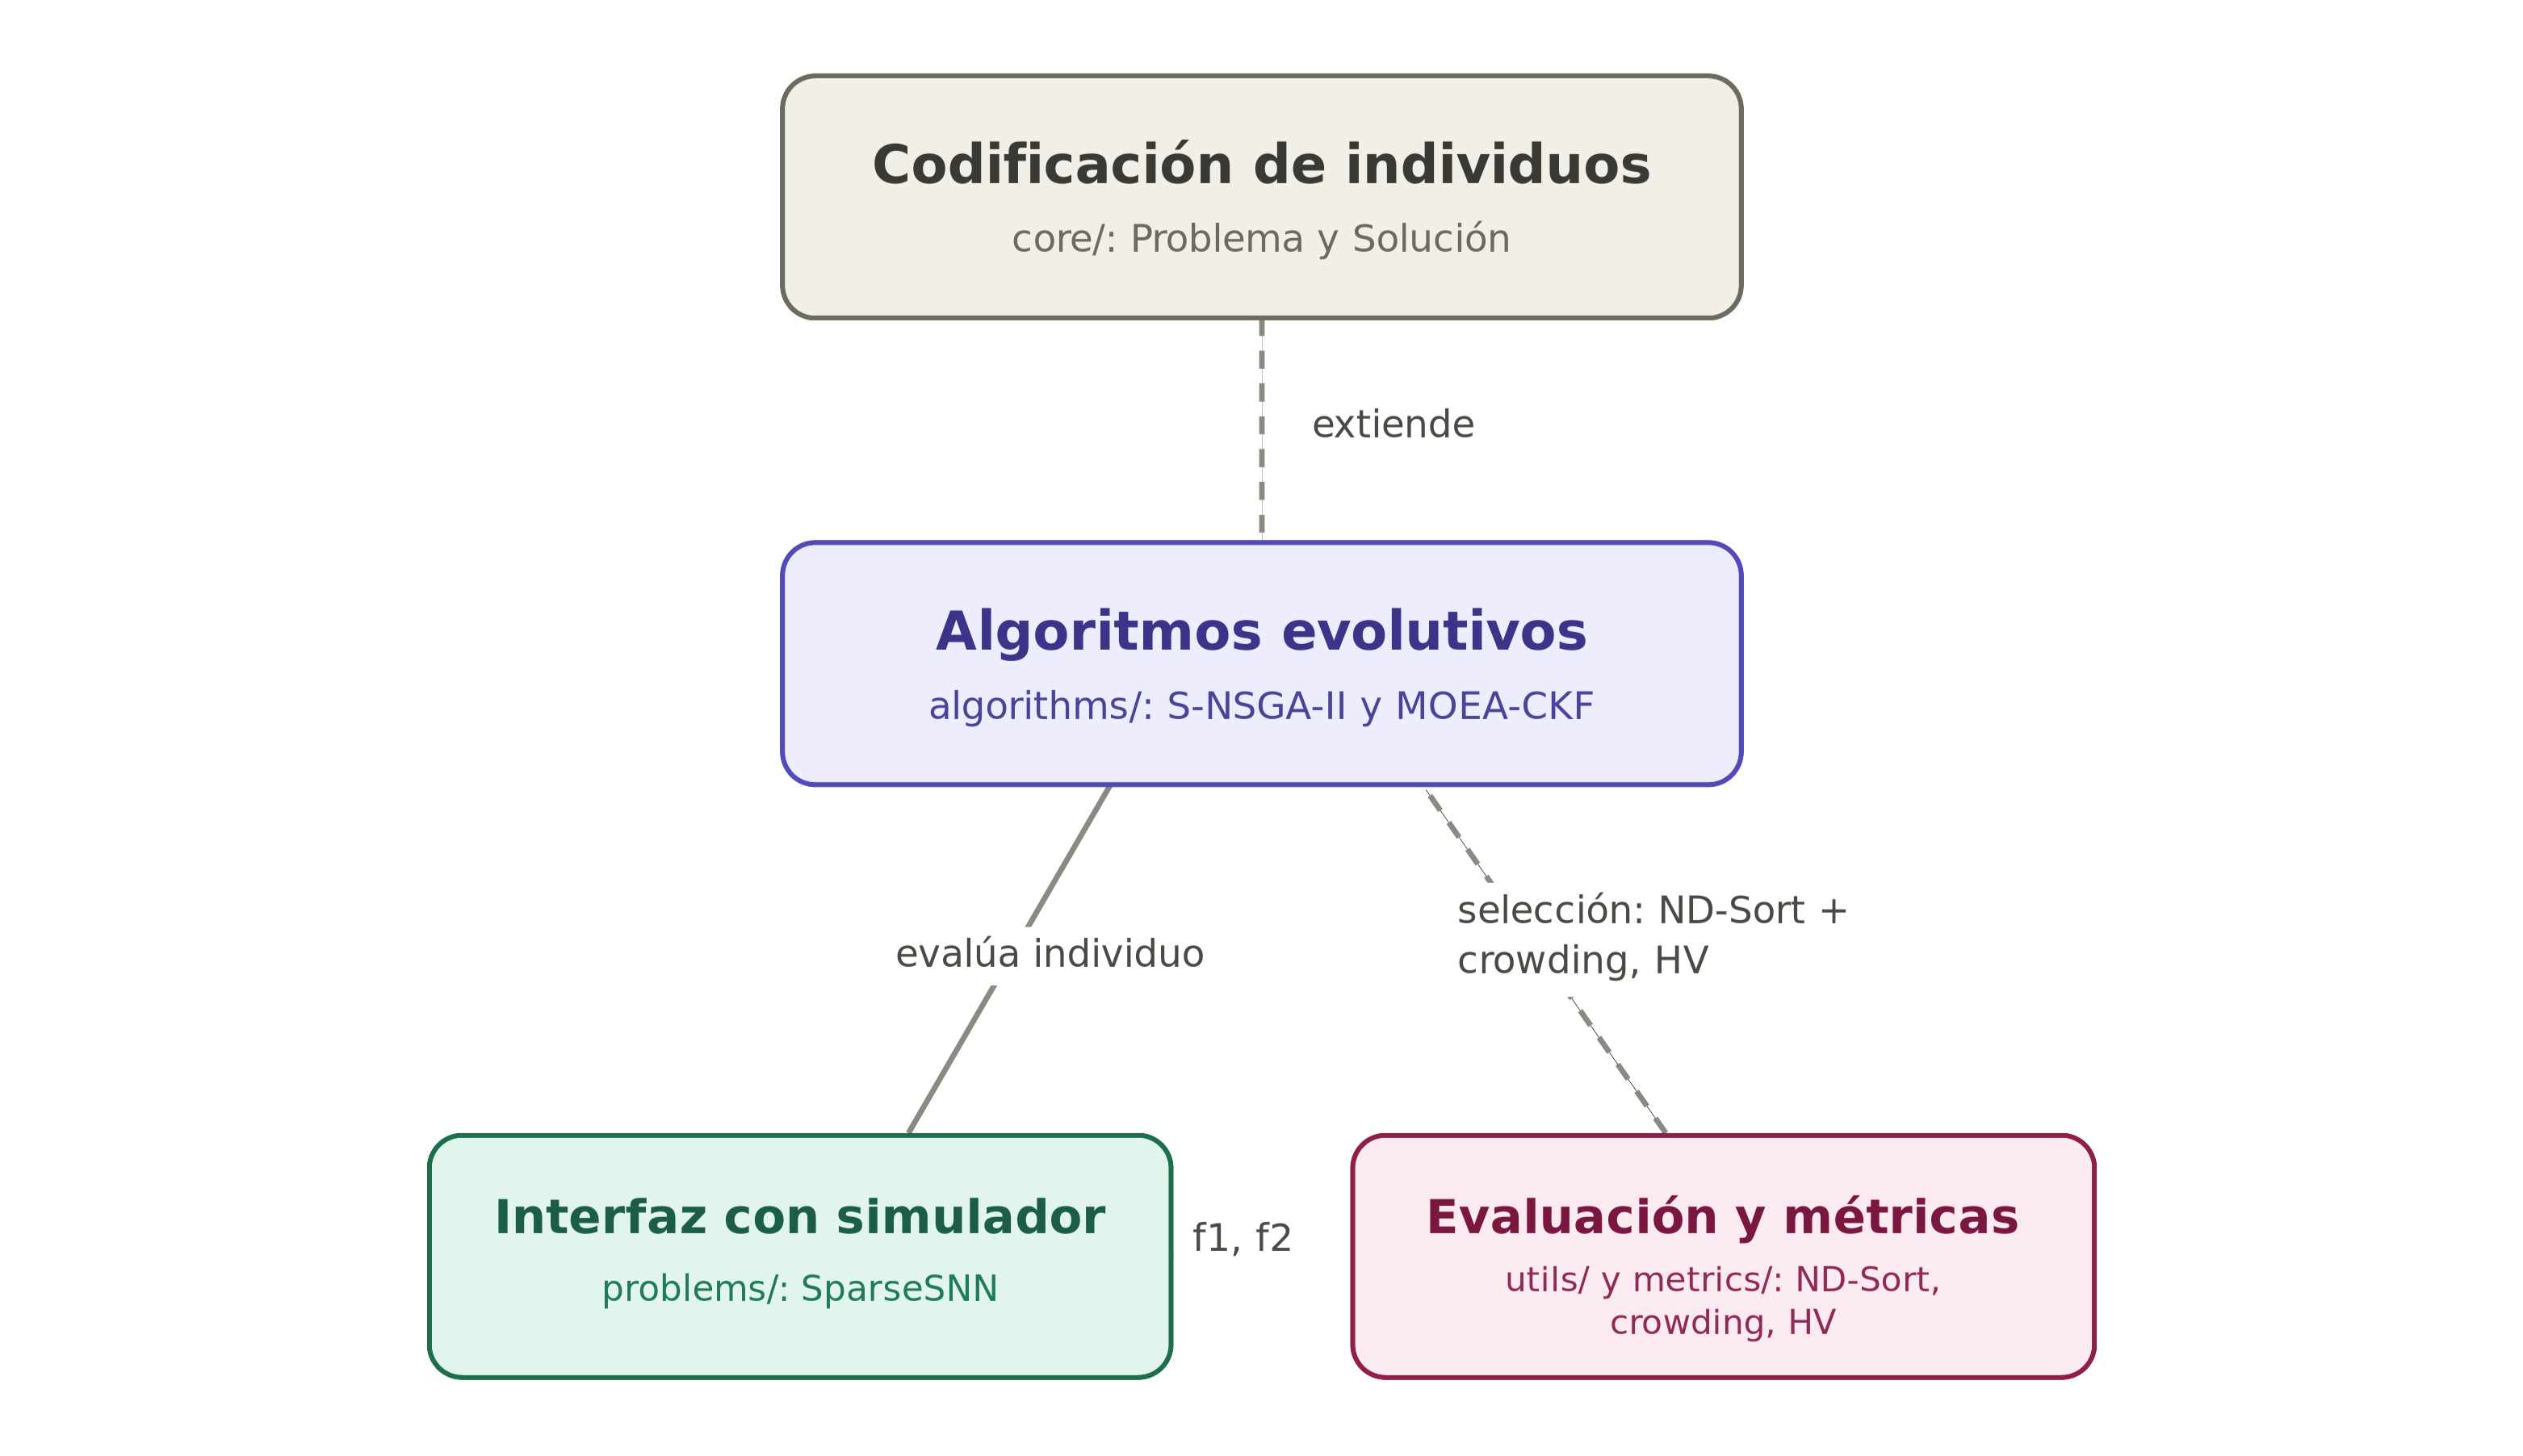
\includegraphics[width=0.75\linewidth]{images/modulos_algoritmos_evolutivos.png}
    \caption{Organización modular del módulo evolutivo.}
    \label{fig:modulos_platemo_cpp}
\end{figure}

La representación de cada individuo consistió en un vector real de pesos sinápticos definidos sobre la topología fija descrita en la Sección \ref{sec:arqui_sistema}. Dado que un peso nulo desactiva efectivamente una sinapsis, el mismo vector codificó implícitamente tanto la presencia o ausencia de cada conexión como la intensidad de las conexiones activas, permitiendo abordar el problema desde un enfoque neuroevolutivo sin requerir un cromosoma de topología independiente. Esta codificación conjunta fue la que permitió optimizar simultáneamente el desempeño de clasificación y la complejidad estructural de la red, los dos objetivos definidos para el problema.

Una vez implementados los algoritmos en C++, estos fueron integrados con el simulador de SNN a través del problema de entrenamiento de SNN. Así, la evaluación de cada individuo consistió en ejecutar una configuración experimental completa definida por un dataset, una cantidad de variables de entrada y un número determinado de neuronas en la capa oculta. Bajo este esquema, cada solución propuesta por el algoritmo evolutivo fue decodificada en una arquitectura de red concreta, simulada sobre los datos correspondientes y evaluada según las funciones objetivo definidas para el problema. Con esto se obtuvo una plataforma experimental unificada, capaz de conectar el proceso evolutivo con la simulación de SNN y de soportar las etapas posteriores de evaluación y comparación de resultados. El proceso de optimización siguió un ciclo iterativo que ya fue explicado en la Sección \ref{sec:arqui_sistema}.

% Finalmente, se verificó que la implementación en C++ preservara la lógica general de los algoritmos de referencia y resultara compatible con la ejecución repetible de experimentos. Para ello, se incorporaron mecanismos de parametrización de los algoritmos, configuración del tamaño de la capa oculta y gestión del dataset a utilizar en cada ejecución. 


%----------------------------
